\subsection{SIP}

As previously noted, the \gls{sip} traffic is not protected by \gls{tls}. The lack of encryption means that an attacker could intercept all calls made and received by the customer and also capture the hashed \gls{sip} password to brute-force it.

The problem is aggravated by the discovery that any customer is able to authenticate to the \gls{sip} server with any phone number as long it has the correct credentials. The server doesn’t check the origin of the request to forbid other customers from having access to numbers that don’t belong to them. In the experiment, shown in Figure \ref{figure:sip_call}, a customer that isn’t subscribed to the \gls{isp} \gls{voip} service and has a copper-based connection, was able to authenticate with a phone number belonging to another customer that has a fiber-based connection and lives 120km apart from where the connection was initiated.

\begin{figure}[h]
    \centering
    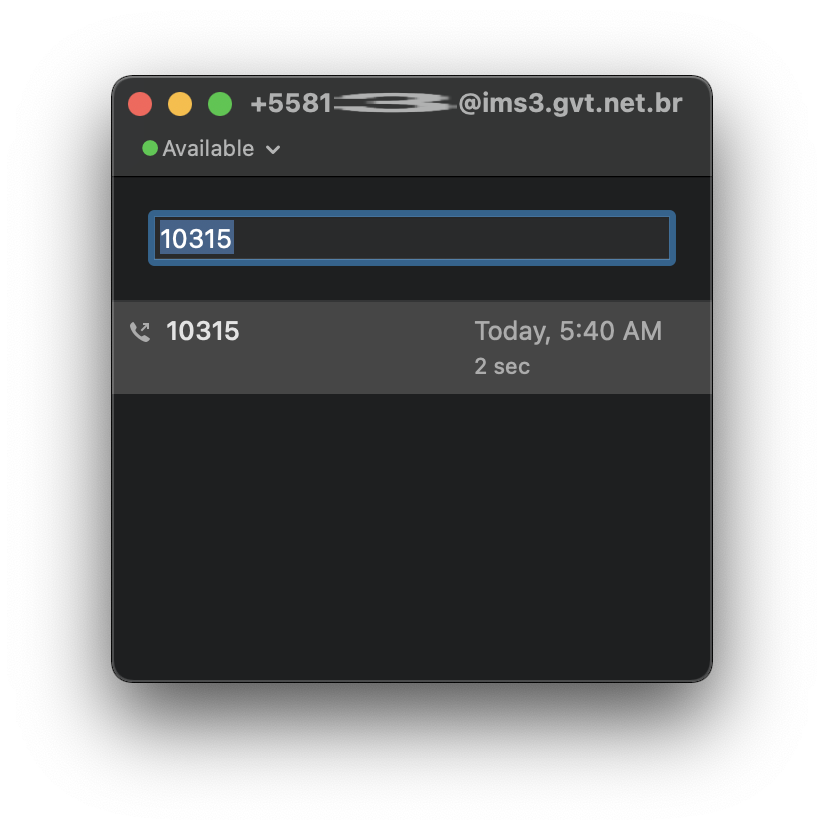
\includegraphics[width=\linewidth]{contents/isp-side-services-analysis/sip/sip-call.png}
    \caption{Call Made Using the Phone Number of Another Customer}
    \label{figure:sip_call}
\end{figure}

It was verified that the \gls{sip} server has another two problems. It allows enumeration of phone numbers that it is able to authenticate, and there is no mechanism in place that prevents online brute-forcing. Using the PJSUA library to open a single connection, it was able to enumerate phones at a speed of 5.67 per second and brute-force passwords at a speed of 1.27 per second. Both attacks can be parallelized as long as the \gls{sip} server is able to handle the throughput of requests.

Enumeration was also found to be possible by trying to register a random number without providing any authorization token. If the phone number is valid, the client receives a 100 Trying response followed by an 401 Unauthorized response, Figure \ref{figure:sip_401}. On the other hand, if the phone doesn’t exist on their database, the response is a 100 Trying followed by a 403 Forbidden, Figure \ref{figure:sip_403}.

\begin{figure}[h]
    \centering
    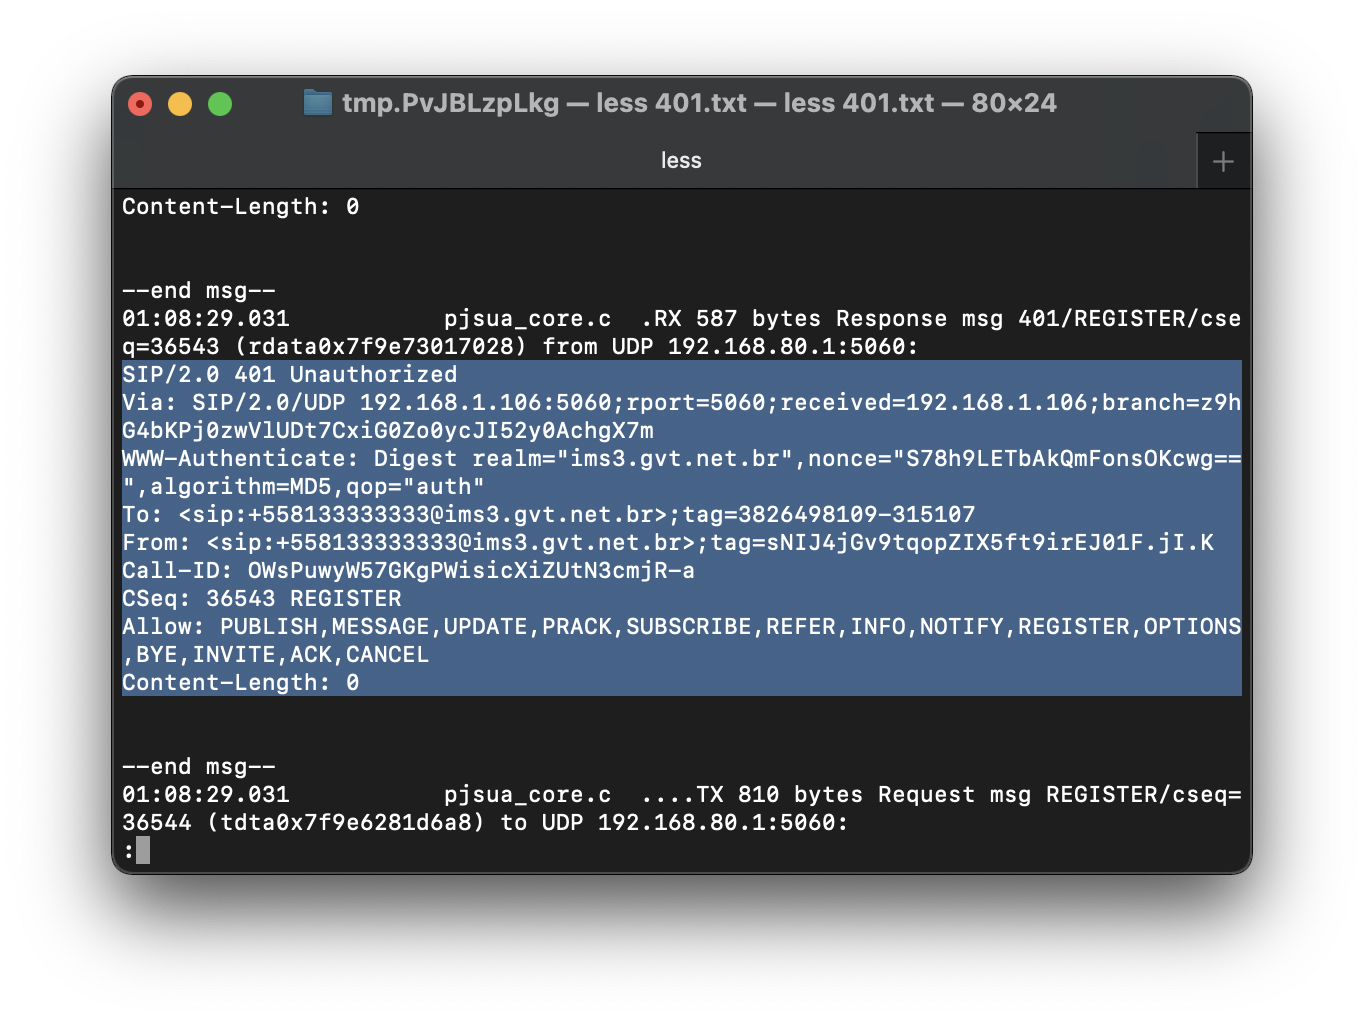
\includegraphics[width=\linewidth]{contents/isp-side-services-analysis/sip/sip-401.png}
    \caption{Unauthorized \gls{sip} Response for Existent Phone Number}
    \label{figure:sip_401}
\end{figure}

\begin{figure}[h]
    \centering
    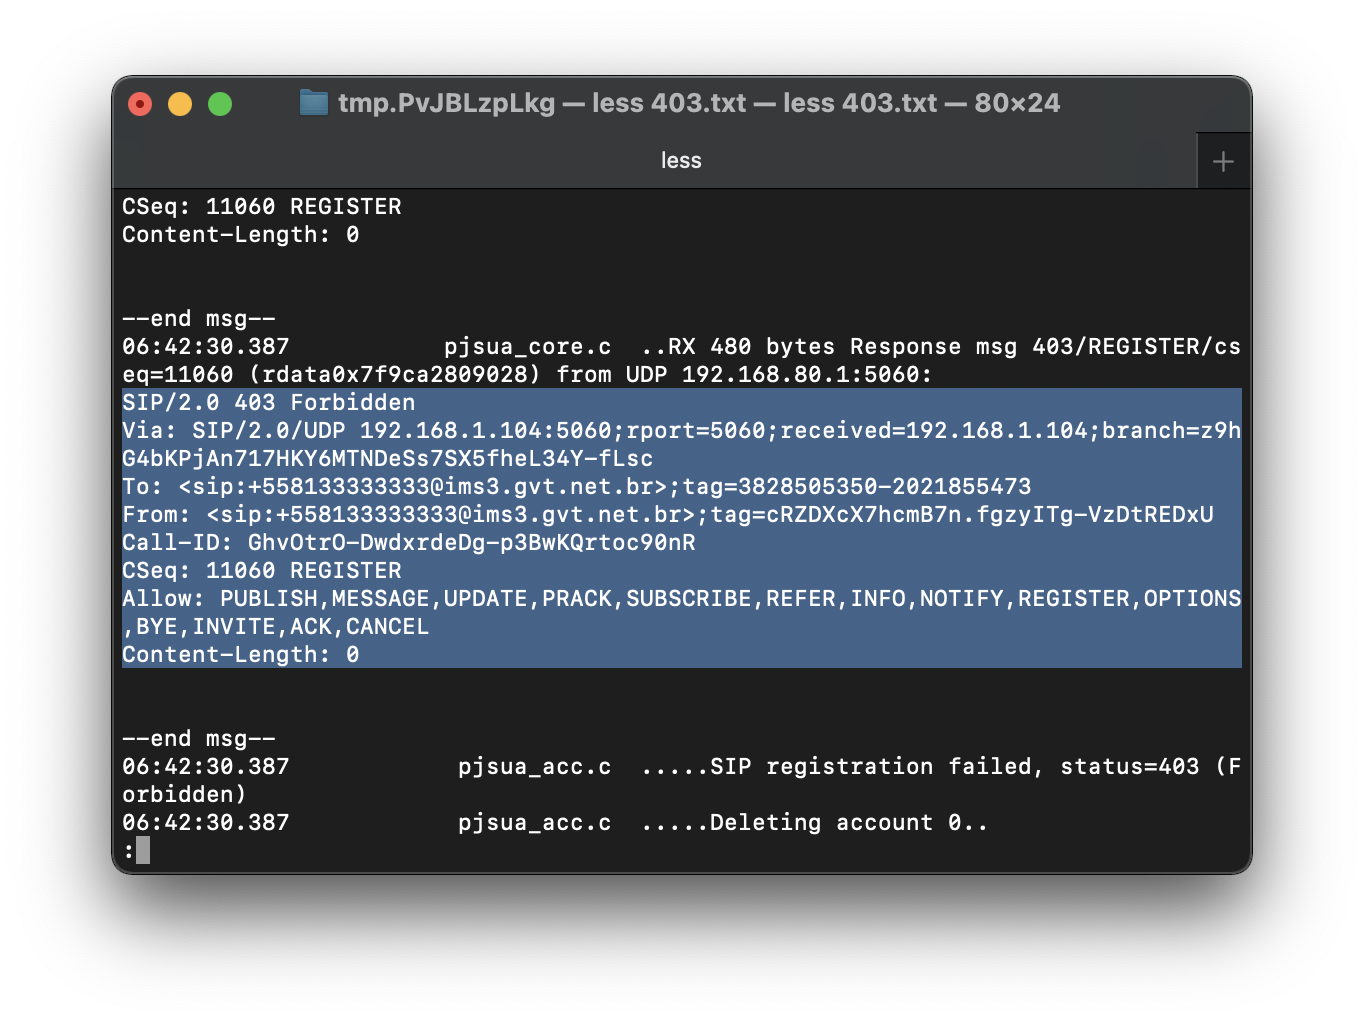
\includegraphics[width=\linewidth]{contents/isp-side-services-analysis/sip/sip-403.png}
    \caption{Forbidden \gls{sip} Response for Nonexistent Phone Number}
    \label{figure:sip_403}
\end{figure}

In regards to online brute-forcing, an attacker is able to guess the password an unlimited number of tries without triggering any protection mechanism on the server. The attack can be distributed and run concurrently without any penalty.

Another critical mechanism that could be exploited by an attacker is the registration process of \gls{sip} credentials on the \gls{cpe}. Unfortunately, none of the experiments performed were able to detect this procedure. The devices don't requests the credentials to the \gls{isp} and the \gls{isp} doesn't send the credentials proactively.

It is speculated that either the \gls{cpe} is installed on the customer's home with the credentials already set, or that the technician is able to trigger some process that makes the \gls{isp} configure the credentials on \gls{cpe} remotely. It also unknown if customer support is able to reconfigure the credentials, what would allow an attacker to impersonate the customer and induce the support to reset the password while the attacker is sniffing the physical transmission medium.

\FloatBarrier
